%%%%%%%%%%%%%%%%%%%%%%%%%%%%%%%%%%%%%%%%%%%%%%%%%%%%%%%%%%%%%%%%%%%%
%%%%% HEADER %%%%%
%%%%%%%%%%%%%%%%%%%%%%%%%%%%%%%%%%%%%%%%%%%%%%%%%%%%%%%%%%%%%%%%%%%%

\documentclass[a4paper, 12pt]{report}


%%%%% Packages %%%%%

	%%%%% Language %%%%% 
\usepackage[frenchb]{babel}
\usepackage[utf8]{inputenc}
\usepackage[T1]{fontenc}
	%%%%% Graphic %%%%%
\usepackage{graphicx}
\usepackage{titlesec}
\usepackage{verbatim}
\usepackage{moreverb}
\usepackage{multicol}


%%%%% Macros %%%%
\newcommand{\HRule}{\rule{\linewidth}{0.5mm}}

%%%%% Modification du titre du chapitre %%%%%
\titleformat{\chapter}[hang]{\bf\huge}{}{0pc}{}



%%%%% Doc's informations %%%%%


%%%%%%%%%%%%%%%%%%%%%%%%%%%%%%%%%%%%%%%%%%%%%%%%%%%%%%%%%%%%%%%%%%%%
%%%%% DOCUMENT %%%%%
%%%%%%%%%%%%%%%%%%%%%%%%%%%%%%%%%%%%%%%%%%%%%%%%%%%%%%%%%%%%%%%%%%%%

\begin{document}

%%%%% Page de garde %%%%
\begin{titlepage}
	\begin{center}

		
\includegraphics[width=0.45\textwidth]{logoUN.png}~\\[2cm]

		\textsc{\LARGE Master 1 Alma}\\[1.5cm]

		% Titre
		\HRule \\[0.5cm]
		{ \textsc{\Large Projet de TP de compilation}\\[0.5cm] }
		\HRule \\[0.5cm]

		\textsc{\Large Conception d'un compilateur d'images SVG}\\[1.5cm]

		% Auteur et Encadrant
		\emph{\'Etudiant :}\\
		Vincent \textsc{Raveneau}\\
		\vspace{0.5cm}
		\emph{Intervenant :} \\
		Beno\^it \textsc{Guédas}
	
		\vfill

		% Bottom of the page
		{\large 10 Avril 2014}

	\end{center}
\end{titlepage}

%%%%% Sommaire %%%%%
\renewcommand{\contentsname}{Sommaire}
\tableofcontents
\newpage

%%%%% Intro %%%%%
\chapter{Présentation du projet}

Afin de mettre en pratique les différents éléments étudiés lors du cours de compilation et des TPs associés, nous avons eu pour tâche de réaliser un compilateur pour un langage permettant de générer des images au format SVG. Bien que les principaux éléments du langage en question nous aient été imposés par le sujet, leur implémentation restait libre et pouvait être réalisée de différentes façons.\\

Le compilateur devait être codé en Ocaml, à l'aide d'ocamllex et d'ocamlyacc, et sa réalisation devait être décomposées en différentes étapes successives. Bien que l'ordre et le contenu de ces étapes soient entièrement libres, cette stratégie avait pour but de nous permettre de nous concentrer sur une tâche à la fois. De plus, celà garantissait que lors du déroulement d'une étape, tous les aspects du langage définis dans les étapes précédantes étaient pleinement fonctionnels et non partiellement implémentés.\\

Ce rapport a donc pour but de présenter le travail que j'ai effectué dans le cadre de ce projet. Une présentation du langage implémenté sera d'abord effectuée, puis chaque étape dans la création du compilateur sera décrite en détail, afin d'illustrer la démarche itérative mise en place.\\

Au cas où le code correspondant ne serait pas présent avec ce document, il est disponible sur un dépôt Git hébergé par GitHub à l'adresse \texttt{https://github.com/Lerian/ProjetTpCompilation} (la section "\textit{releases}" contient une release par étape du projet décrite plus loin dans ce rapport).

%%%%% Présentation du langage %%%%%
\chapter{Présentation du langage implémenté}

	\section{Caractéristiques}
	
	Le langage implémenté doit permettre à l'utilisateur de décrire une image au format SVG. Pour celà, il dispose d'un langage de type impératif, dont la syntaxe est similaire au C. Le typage des variables est implicite, et les opérations entre éléments de types différents sont impossibles (par exemple l'addition d'un entier avec un flottant).
	
	\section{Syntaxe}
	
	\subsection{\'Elements importants}
	
	Les principaux éléments du langage défini sont les suivants:\\
	
	\begin{itemize}
		\item Chaque instruction doit se terminer par un point-virgule
		\item Le caractère \# permet de commenter tout ce qui suit sur une même ligne
		\item L'opérateur d'affectation est \texttt{:=}
		\item Les types primitifs disponibles sont les entiers, les flottants, les booléens, les chaînes de caractères et les couleurs
		\item Les types complexes disponibles sont les points, les lignes, les cercles, les rectangles les image et les textes (qui diffèrent des chaînes de caractères par le fait qu'ils possèdent une représentation graphique)
		\item Les opérateurs sur les types primitifs ne peuvent s'appliquer à des types différents (\texttt{0 + 0.0} est incorrect)
		\item Les caractères d'espacement sont toujours ignorés entre les différents éléments syntaxiques du langage
		\item La primitive de dessin est \texttt{draw}, et prend en argument l'image et la forme à dessiner
	\end{itemize}
	
	\subsection{Exemple de code valide}
	
	Le code suivant est un code valide:
	
	\begin{verbatim}
	demonstration := Image(400,400);

	ligneH := Line(0.0,200.0,400.0,200.0);
	ligneV := Line(200.0,00.0,200.0,400.0,blue,3);
	rectangle := Rectangle(0.0,0.0,400.0,200.0,black,yellow,1);

	cercle := Circle(200.0,200.0,50.0); # Un cercle central
	texte := Text("Image de démonstration",125.0,140.0,red,15);

	draw demonstration rectangle;
	draw demonstration ligneV;
	draw demonstration ligneH;
	draw demonstration cercle;
	draw demonstration texte;
	\end{verbatim}
	
	L'image générée par ce code est la suivante:\\
	
	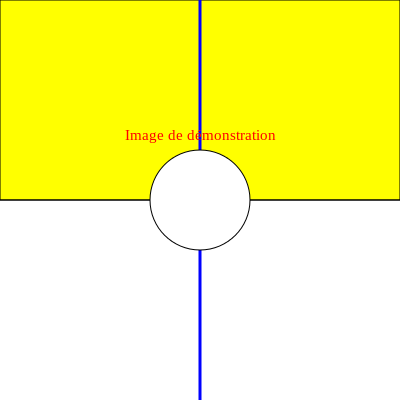
\includegraphics{demonstration.png}~\\
	
	\section{\'Eléments non implémentés}
	
	Bien que demandés par le sujet, certains éléments principaux du langage n'ont pas été implémentés faute de temps. C'est le cas notamment de la gestion des erreurs, et des structures de contrôle telles que les boucles et les conditionnelles (de type \texttt{if (condition) then (instructions) else (instructions)}). Dans le cas de la gestion d'erreur, l'implémentation actuelle lève une exception, généralement \texttt{Not\_found}, ce qui interrompt la compilation dans tous les cas. L'accès aux champs des types complexes par notation pointée est également manquant.

%%%%% Etape 1 %%%%%
\chapter{\'Etape 1 : Types primitifs}
    
    Lors de cette étape initiale, l'objectif était de permettre au compilateur de détecter les types primitifs du langage, qui sont les suivants:\\
    
    \begin{itemize}
    	\item Les entiers : une suite de chiffres allant de 0 à 9;
    	\item Les flottants : un entier suivi d'un point et d'un autre entier. La présence d'au moins un chiffre de chaque côté du point est obligatoire;
    	\item Les cha\^ines de caractères : une suite de caractères encadrée par des guillemets droits (\texttt{"});
    	\item Les booléens : deux valeurs possibles, \texttt{true} et \texttt{false};
    	\item Les couleurs : six couleurs possibles, \texttt{red}, \texttt{blue}, \texttt{yellow}, \texttt{green}, \texttt{black} et \texttt{white}.\\
    \end{itemize}
    
    Leur définition par l'analyseur lexical est donc la suivante:
    
    \begin{verbatimtab}[4]
    	let blank = [' ' '\t' '\r']
		let digit = ['0'-'9']
		let letter = ['a'-'z']|['A'-'Z']

		(** Types primitifs *)
		let flottant = digit+'.'digit+
		let entier = digit+
		let couleur = "red"|"blue"|"yellow"|"green"|"black"|"white"
		let booleen = "true"|"false"
		let chaineCaracs =  [^'"']*
    \end{verbatimtab}
    
    \`A partir de cette étape du projet et jusqu'à l'implémentation des variables et des fonctions de dessin, lorsqu'un élément correspondant à un de ces types est identifié, son type et sa valeur sont affichés sur la sortie standard mais aucune action n'est effectuée dessus.\\
    
    Lors de cette étape, la prise en compte des commentaires a également été mise en place. Ceux-ci sont similaires à ceux que l'on peut trouver en Python, et se caractérisent par le caractère \texttt{\#}. Tout caractère situé après lui sur la même ligne est ignoré par le compilateur.\\
    
%%%%% Etape 2 %%%%%
\chapter{\'Etape 2 : Opérations sur les types primitifs}

	Une fois les types primitifs intégrés, les opérateurs usuels correspondant ont été implémentés. Ceux-ci peuvent être de trois sortes, selon les types auxquels ils s'appliquent.\\
	
	Tout d'abord, les opérateurs arithmétiques ont été mis en place. Ceux-ci sont l'addition (\texttt{+}), la soustraction (\texttt{-}), la multiplication (\texttt{*}), la division (\texttt{/}) et le modulo (\texttt{\%}). Ces opérateurs s'appliquent aux entiers et aux flottants, à l'exception du modulo qui ne s'applique par définition qu'aux entiers. Il est cependant important de noter que les deux opérandes associées à un opérateur doivent être de même type (par exemple, l'addition d'un entier avec un flottant est impossible).\\

	Ensuite, les opérateurs de comparaison ont été  implémentés. Ceux-ci s'appliquent également aux entiers et au flottants, et les opérandes d'un opérateur doivent toujours être de même type. On trouve les opérateurs d'infériorité stricte (\texttt{<}), de supériorité stricte (\texttt{>}), d'infériorité (\texttt{<=}) et de supériorité (\texttt{=>}).\\
	
	Enfin, les opérateurs booléens de composition ont été mis en place. Ceux-ci sont le ET logique (\texttt{and}) et le OU logique (\texttt{or}), et s'appliquent aux booléens comme leur nom l'indique. Le OU est ici non-exclusif, ce qui signifie que l'expression \texttt{vrai ou vrai} a pour valeur \texttt{vrai}.\\
	
	La prise en compte des parenthèses afin de définir les priorités dans le calcul des expressions a également été mise en place pour les trois catégories d'opérateurs décrites ci-dessus. Leur utilisation est effectuée en notation infixée (\textit{operande1 operateur operande2}), les caractères d'espacement entre les opérandes et l'opérateur étant ignorés par le compilateur.
    
%%%%% Etape 3 %%%%%
\chapter{\'Etape 3 : Types complexes basiques}

	Après avoir fait en sorte que les types primitifs soient pleinement gérés par le compilateur, il a été nécessaire d'implémenter les types dits "complexes". Ces types s'apparentent aux structures que l'ont peut trouver en C, et sont composés de différents champs ayant chacun un type particulier (le type en question peut être primitif ou complexe). Ces types ont été implémentés en deux étapes. En effet, ils comportent des champs dont la valeur permet de personnaliser l'apparence des objets (en déterminant par exemple la couleur d'un texte). Les champs indispensables ont tous été implémentés dans cette étape, ce qui m'a permis d'avoir des objets fonctionnels pour commencer à mettre en place les champs optionnels dans l'étape suivante.\\
	
	Les types complexes implémentés sont les suivants:\\
	
	\begin{itemize}
		\item Le cercle, composé d'un point central et d'un rayon (un flottant);
		\item Le rectangle, composé du point de son extrémité haute/gauche, d'une largeur (un flottant) et d'une hauteur (un flottant);
		\item La ligne, composée de deux points pour ses extrémités;
		\item Le texte, composé du point de son extrémité basse/gauche et de la cha\^ine de caractères correspondante;
		\item L'image, composée d'une largeur (un entier) et d'une hauteur (un entier).\\
	\end{itemize}
	
	De plus, afin de simplifier la structure de tous les types nécessitant un point, un type \texttt{Point} à été créé, qui contient les coordonnées associées (deux flottants).\\
	
	Ces différents types ont été définis par des enregistrements, qui sont de la forme suivante (à l'exception de l'image, dont les champs n'ont pas l'attribut \texttt{mutable} étant donné qu'ils ne peuvent être modifiés):\\
	
	\begin{verbatimtab}[4]
	type rectangle = {
		mutable r_coinHG: point;
		mutable r_width: float;
		mutable r_height: float
	}
	\end{verbatimtab}
	
	Pour créer des instances de ces types, il est nécessaire d'utiliser des constructeurs, qui prennent pour paramètre toutes les valeurs des champs du type. Ceux-ci sont de la forme \textit{nomDuType(param1 , param2)}, avec le nombre de paramètres pouvant varier d'un type à l'autre. Tous les caractères d'espacement présents sont ignorés. Il faut cependant noter que dans le cas d'un point, les constructeurs prennent deux valeurs correspondant aux coordonnées du point en question, et non une instance de Point. Ainsi, les constructeurs disponibles sont les suivants:\\
	
	\begin{itemize}
		\item Pour le cercle : \textit{Circle(centre\_x, centre\_y, rayon)}
		\item Pour le rectangle : \textit{Rectangle(coin\_x, coin\_y, largeur, hauteur)}
		\item Pour la ligne : \textit{Line(x1, y1, x2, y2)}
		\item Pour le texte : \textit{Text(contenu, coin\_x, coin\_y)}
		\item Pour le image : \textit{Image(largeur, hauteur)}
		\item Pour le point : \textit{Point(x, y)}\\
	\end{itemize}
	
	\`A cette étape, les valeurs appliquées par le constructeur aux champs de l'instance du type créée ne sont pas modifiables. En effet, le sujet demandais un accès aux différents champs par notation pointée, mais son implémentation n'était pas possible avant la mise en place de variables pour mémoriser les valeurs ainsi créées.
        
%%%%% Etape 4 %%%%%
\chapter{\'Etape 4: Types complexes évolués}

	Comme dit dans la description de l'étape précédante, les types complexes possèdent des champs optionnels destinés à paramétrer l'apparence des objets créés. Ces champs ont été implémentés dans cette étape du projet, et sont les suivants:\\
	
	\begin{itemize}
		\item Le cercle et le rectangle possèdent une épaisseur de contour (un entier, par défaut à 1), une couleur de remplissage (une couleur, par défaut à \texttt{white}) et une couleur de contour (une couleur, par défaut à \texttt{black});
		\item La ligne possède une épaisseur de contour (un entier, par défaut à 1) et une couleur de contour (une couleur, par défaut à \texttt{black});
		\item Le texte possède une couleur d'écriture (une couleur, par défaut à \texttt{black}) et une taille de fonte (un entier, par défaut à 12).\\
	\end{itemize}
	
	Afin de permettre à l'utilisateur de modifier les valeurs de ces champs, les constructeurs définis lors de l'étape précédante ont été modifiés afin de demande en plus des paramètres obligatoires les paramètres optionnels. Dans le cas où l'utilisateur ne fournirait que les paramètres obligatoires, le compilateur se charge de compléter l'appel au constructeur avec les valeurs par défaut appropriées. Concernant les paramètres optionnels, ils doivent tous être présents ou bien tous être absents, ne fournir qu'une partie d'entre eux au constructeur déclenche une erreur. La nouvelle forme des constructeurs est donc la suivante:\\
	
	\begin{itemize}
		\item Pour le cercle : \textit{Circle(centre\_x, centre\_y, rayon, couleurContour, couleurRemplissage, epaisseurContour)}
		\item Pour le rectangle : \textit{Rectangle(coin\_x, coin\_y, largeur, hauteur, couleurContour, couleurRemplissage, epaisseurContour)}
		\item Pour la ligne : \textit{Line(x1, y1, x2, y2, couleurContour, epaisseurContour)}
		\item Pour le texte : \textit{Text(contenu, coin\_x, coin\_y, couleur, tailleFonte)}
	\end{itemize}
	
%%%%% Etape 5 %%%%%
\chapter{\'Etape 5 : Variables et instructions}

	\`A ce stade, toutes les fonctionnalités nécessaires à la création d'une image sont présentes et fonctionnelles, à l'exception de la prise en compte des variables, et de l'instruction de dessin elle-même. Cette étape aura donc pour but de mettre ceci en place, afin de produire les premiers fichiers SVG. Pour faciliter la gestion des différentes instructions qui allaient devoir être prises en compte, c'est à ce moment qu'à été mise en place l'obligation de terminer chaque instruction par un point-virgule, comme demandé par le sujet.\\
	
	Une première version avait d'abord été réalisée, dans laquelle on distinguait deux étapes distinctes pour l'analyseur syntaxique et l'analyseur sémantique, avec la construction d'un arbre syntaxique abstrait par le premier qui était utilisé par le second. Cependant, le temps nécessaire à sa mise en place était trop important (de nombreuses modifications devant être effectuées sur la structure du compilateur), c'est pourquoi ces deux étapes sont réunies en une seule dans l'implémentation actuelle.
	
	\section{Les variables}
	
	Les variables permettent de mémoriser des valeurs de types primitifs ou complexes qui leur sont affectées. Cette opération est effectuée par l'opérateur d'affectation \texttt{:=}. Le nom d'une variable est composé d'une suite de lettres (minuscules et majuscules), de chiffres et du caractère '\_', mais doit commencer par une lettre.\\
	
	Une première tentative a été réalisée, où chaque type de variable était stocké dans une table qui lui était propre, mais cette implémentation demandait de trop nombreux tests sur les types avant le moindre accès à une variable, ce qui rendait le code lourd et peu pratique. De plus, vérifier qu'une nouvelle variable n'était pas déjà déclarée dans la table d'un autre type était fastidieux. C'est pour cette raison que la façon dont les variables sont gérées a été modifiée afin d'arriver à l'implémentation décrite dans les paragraphes suivants.\\
	
	Le compilateur enregistre les variables déclarées dans une Hashtbl, qui associe une cha\^ine de caractères (le nom de la variable) à un couple composé du type et de la valeur de la variable. \`A chaque fois qu'une affectation est réalisée, le compilateur vérifie si la variable correspondante est présente dans la table ou non. Si c'est le cas, il vérifie que le type associé est respecté, puis met à jour la valeur. Sinon, la variable, sa valeur et son type sont ajoutés à la table. Les variables de type image agissent cependant de façon légèrement différente. En effet, comme elles ne peuvent être modifiées, l'affectation échoue si la variable existe déjà dans la table.\\
	
	Afin de pouvoir construire une table telle que décrite ci-dessus, qui puisse stocker des variables de différents types, les deux types suivants ont dû être définis:

\begin{multicols}{2}
\begin{verbatimtab}[4]
	type type_t_values =
		|Entier_t
		|Flottant_t
		|Booleen_t
		|Chaine_t
		|Couleur_t
		|Cercle_t
		|Rectangle_t
		|Ligne_t
		|Texte_t
		|Image_t
		|Point_t
		
	type type_t =
		|Entier of int
		|Flottant of float
		|Booleen of bool
		|Chaine of string
		|Couleur of string
		|Cercle of cercle
		|Rectangle of rectangle
		|Ligne of ligne
		|Texte of texte
		|Image of image
		|Point of point
\end{verbatimtab}
\end{multicols}
	
	Lors de l'accès à une variable, le compilateur récupère simplement dans la table la valeur associée. La récupération de la valeur d'une variable d'un type donné étant effectuée par une fonction différente de celle permettant la récupération d'une valeur d'un autre type, une vérification sur la concordance du type de la valeur retournée est également effectuée. Un exemple d'une telle fonction est le suivant:
	
\begin{verbatimtab}[4]
	let get_float_value varName =
	begin
		if(Hashtbl.mem variables varName)
		then
			match Hashtbl.find variables varName with
				|	(Flottant_t, Flottant x)	->	x
				|	_				->	raise Not_found
				;
		else
				raise Not_found
	end
\end{verbatimtab}

	Le comportemant si la variable est de type \texttt{Image} est légèrement différent, et sera décrit dans la partie suivante, consacrée à la primitive de dessin.

	\section{La primitive de dessin}
	
	La primitive de dessin \texttt{draw} prend en paramètres deux variables, une de type \texttt{Image} et l'autre d'un type correspondant à une forme dessinable (cercle, rectangle, texte ou ligne). La forme donnée est ainsi ajoutée à l'image, afin d'être dessinée dans le fichier SVG produit.\\
	
	Pour chaque variable de types \texttt{Image}, un fichier est créé (nommé \textit{nomDelaVariable.svg}) une fois que toutes les instructions du programme ont été exécutées. Lors de leur exécution, la valeur du fichier est stockée dans une deuxième table qui associe au nom de la variable le contenu du fichier correspondant. Chaque appel à la primitive de dessin concatène donc la valeur actuelle associée avec la description de la forme donnée.\\
	
	Une fois toutes les instructions exécutées, cette table est parcourue et tous les fichiers correspondant sont créés. Cette solution permet de limiter les opérations d'ouverture/fermeture de fichiers, comparé à une solution où à chaque appel à la primitive de dessin le contenu du fichier aurait été modifié.\\
	
	Afin de mettre en place le dessin des variables de type \texttt{Texte}, la façon dont les chaînes de caractères étaient reconnues par l'analyseur lexical a dû être modifiée afin que les guillements identifiant une telle structure n'apparaissent pas systématiquement dans le dessin final.

\end{document}
